\subsection{Rancangan Detail Komponen Service}
\label{sec:rancangan-service}

Berdasarkan \textit{sequence diagram} yang telah dibuat pada bagian \ref{subsec:arsitektur-behavioural}. Sistem \textit{service} akan dibagi menjadi beberapa domain. Pembagian domain berfungsi untuk memfokuskan implementasi serta memudahkan tahapan testing. Terdapat 6 domain yaitu \textit{company}, \textit{user}, \textit{devices}, \textit{groups}, \textit{deployment}, dan \textit{external services}. Setiap domain akan memiliki diagram kelas yang menjelaskan rancangan implementasi. \textit{package} diagram dan \textit{class} diagram secara keseluruhan dapat dilihat pada gambar \ref{fig:package-diagram} dan \ref{fig:package-class-domain-diagram}
\begin{figure}[ht]
  \centering
  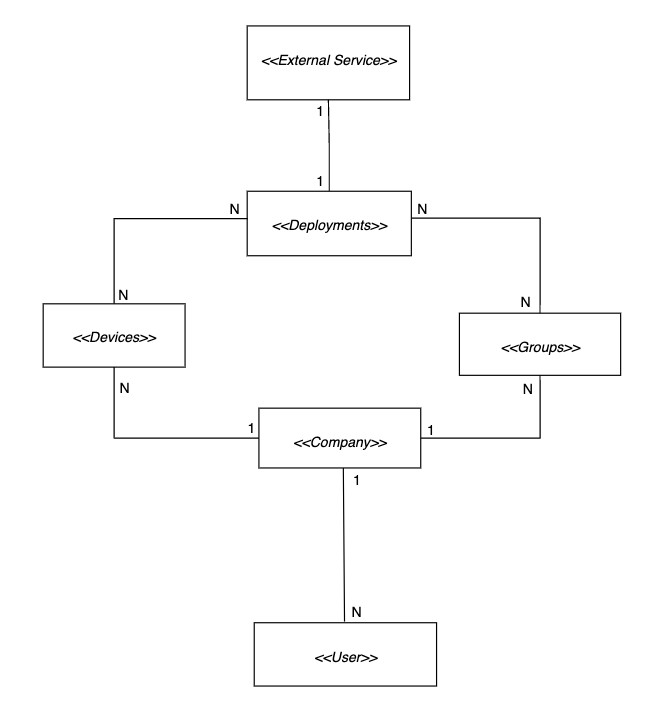
\includegraphics[width=1\textwidth]{resources/chapter-3/class/class-diagram-overall.jpg}
  \caption{\textit{Package Diagram Domain Service}}
  \label{fig:package-class-domain-diagram}
\end{figure}

\begin{figure}[ht]
  \centering
  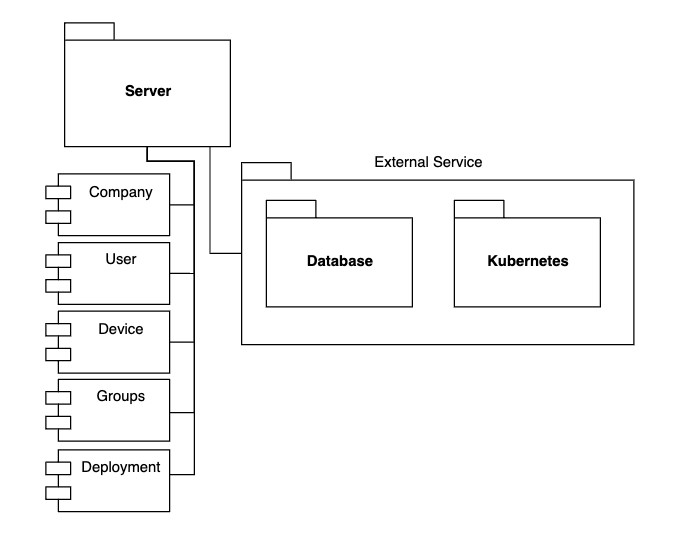
\includegraphics[width=1\textwidth]{resources/chapter-3/package-backend-diagram.jpg}
  \caption{\textit{Package Diagram} Komponen \textit{Service}}
  \label{fig:package-diagram-backend}
\end{figure}

\subsubsection{Domain \textit{company}}

Domain ini mengatur konektivitas antara server dan database dalam hal \textit{company}. Domain ini memiliki tiga lapisan yaitu \textit{handler, usecase, dan repository}. Lapisan \textit{repository} yang akan melakukan hubungan dengan database dan lapisan \textit{handler} yang akan berinteraksi dengan request yang masuk.

\begin{figure}[ht]
  \centering
  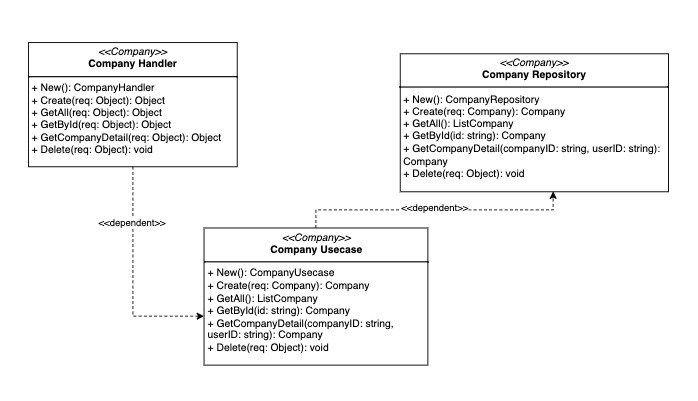
\includegraphics[width=1\textwidth]{resources/chapter-3/class/company-class-diagram.jpg}
  \caption{\textit{Company Class Diagram}}
  \label{fig:company-class-diagram}
\end{figure}

\pagebreak

\subsubsection{Domain \textit{user}}

Domain ini mengatur konektivitas antara server dan database dalam hal \textit{user}. Domain ini juga memliki tiga lapisan mulai dari lapisan paling luar \textit{handler}, diikuti dengan \textit{usecase} lalu terkahir \textit{repository} yang berhubungan dengan database. Domain ini juga yang mengatur bagian autentikasi seperti login dan register.

\begin{figure}[ht]
  \centering
  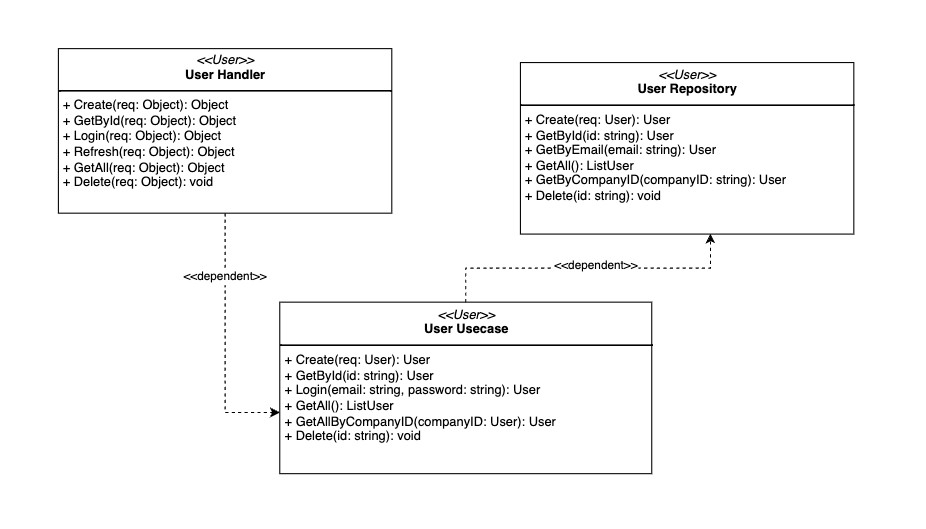
\includegraphics[width=1\textwidth]{resources/chapter-3/class/user-class-diagram.jpg}
  \caption{\t\textit{User Class Diagram}}
  \label{fig:user-class-diagram}
\end{figure}

\subsubsection{Domain \textit{devices}}

Domain ini mengatur perangkat yang ada dalam sistem. Setiap perangkat memiliki ikatan dengan \textit{company}. Domain ini mengatur masalah CRUD dari satu \textit{company} yang dapat di manage oleh banyak \textit{user}. Sama seperti domain lainnya, domain ini memiliki tiga lapisan yaitu \textit{handler, usecase, dan repository}.

\begin{figure}[ht]
  \centering
  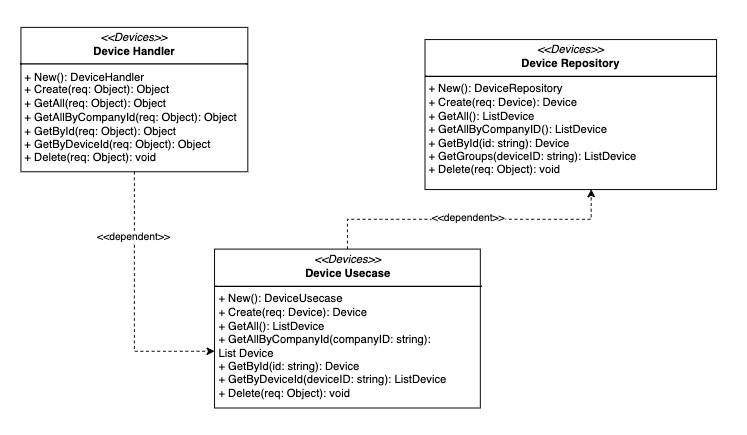
\includegraphics[width=1\textwidth]{resources/chapter-3/class/device-class-diagram.jpg}
  \caption{\textit{Device Class Diagram}}
  \label{fig:device-class-diagram}
\end{figure}

\subsubsection{Domain \textit{groups}}

Domain ini mengatur \textit{groups} yang merupakan gabungan dari satu atau lebih perangkat. Seperti domain \textit{devices}, domain ini pun dapat dikelompokan berdasarkan \textit{company}. Seluruh \textit{user} dapat manage \textit{groups} selama masih dalam satu perusahaan yang sama. Domain ini juga memiliki tiga lapisan yaitu \textit{handler, usecase, dan repository}

\begin{figure}[ht]
  \centering
  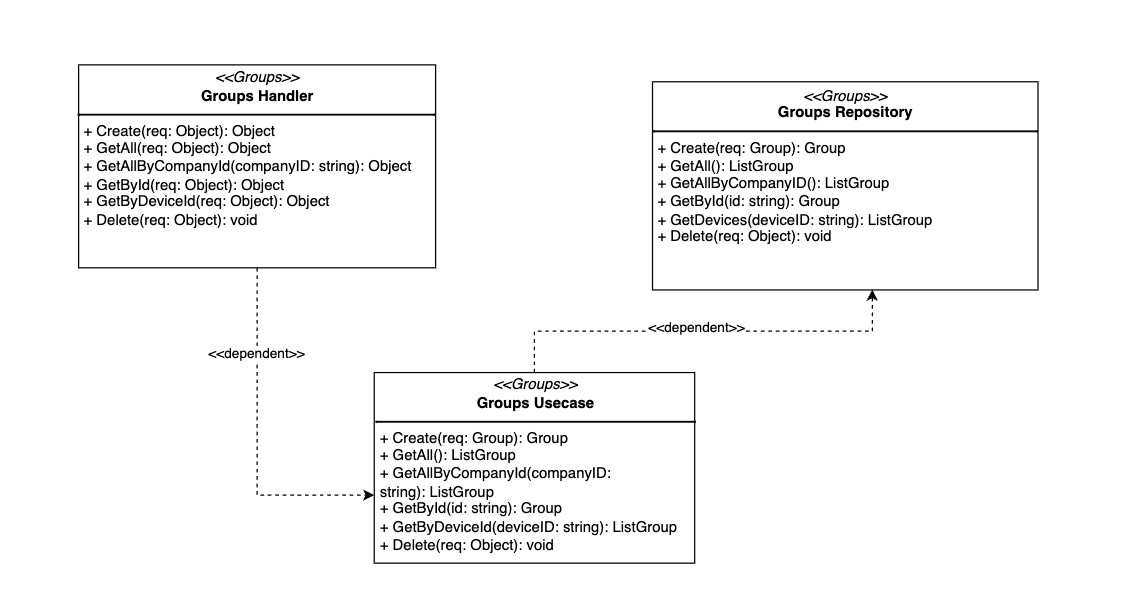
\includegraphics[width=1\textwidth]{resources/chapter-3/class/groups-class-diagram.jpg}
  \caption{Groups \textit{Class Diagram}}
  \label{fig:groups-class-diagram}
\end{figure}

\pagebreak

\subsubsection{Domain \textit{deployment}}

Domain ini merupakan domain yang paling \textit{complex} pada service ini. Domain ini cukup luas karena berhubungan dengan \textit{deployment images} dan \textit{deployment history}. Selain itu domain ini juga memiliki hubungan dengan external service yaitu \textit{kubernetes} untuk proses deploymentnya.

\begin{figure}[ht]
  \centering
  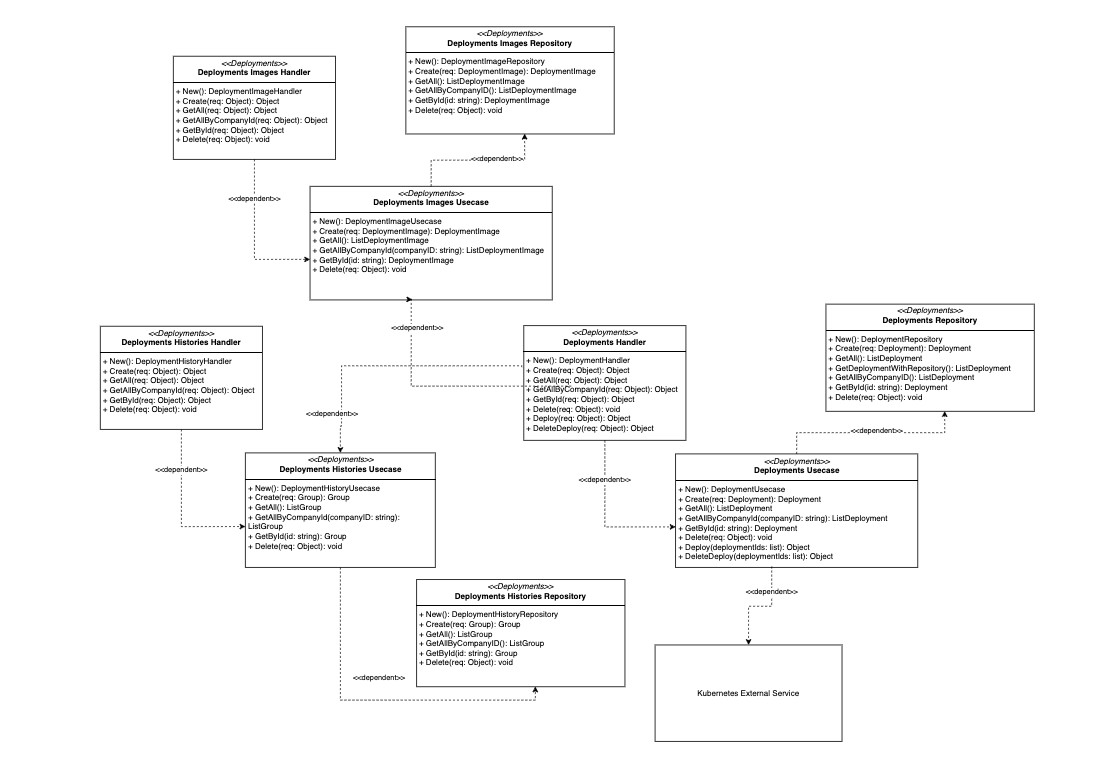
\includegraphics[width=1\textwidth]{resources/chapter-3/class/deployment-class-diagram.jpg}
  \caption{Deployment \textit{Class Diagram}}
  \label{fig:deployment-class-diagram}
\end{figure}

\subsubsection{Domain \textit{external services}}

Domain ini merupakan sebuah interface dari \textit{external service} yang digunakan oleh sistem. Terdapat dua external service yaitu \textit{database} dan \textit{kubernetes}. Namun,

\begin{figure}[ht]
  \centering
  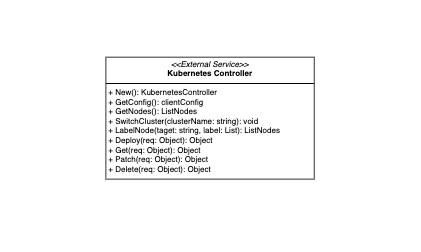
\includegraphics[width=0.7\textwidth]{resources/chapter-3/class/kubernetes-controller}
  \caption{Kubernetes Controller \textit{Class Diagram}}
  \label{fig:kubernetes-controller-class-diagram}
\end{figure}